\documentclass[12pt,a4paper]{article}

% ===================== GÓI LỆNH =====================
\usepackage[a4paper,top=2.5cm,bottom=2.5cm,left=3cm,right=2cm]{geometry}
\usepackage{fontspec}
\setmainfont{Times New Roman}
\usepackage{polyglossia}
\setmainlanguage{vietnamese}

% \usepackage{titlesec} % Commented out due to package not being available
\usepackage{enumitem}
\usepackage{graphicx}
\usepackage{array}
\usepackage{longtable}
\usepackage{booktabs}
\usepackage{xcolor}
\usepackage[hidelinks]{hyperref}
\usepackage{fancyhdr}
\usepackage{multicol}
\usepackage{tabularx}
\usepackage{amssymb}
\usepackage{listings}

% ===================== MÀU SẮC =====================
\definecolor{cmcblue}{RGB}{0,86,163}
\definecolor{cmclight}{RGB}{235,242,250}

% ===================== ĐỊNH DẠNG TIÊU ĐỀ =====================
% Custom section formatting without titlesec
\makeatletter
\renewcommand\section{\@startsection {section}{1}{\z@}%
                                   {-3.5ex \@plus -1ex \@minus -.2ex}%
                                   {2.3ex \@plus.2ex}%
                                   {\normalfont\Large\bfseries\color{cmcblue}}}
\renewcommand\subsection{\@startsection{subsection}{2}{\z@}%
                                     {-3.25ex\@plus -1ex \@minus -.2ex}%
                                     {1.5ex \@plus .2ex}%
                                     {\normalfont\large\bfseries\color{cmcblue}}}
\makeatother

% ===================== HEADER/FOOTER =====================
\pagestyle{fancy}
\setlength{\headheight}{14pt}
\fancyhf{}
\renewcommand{\headrulewidth}{0.4pt}
\fancyhead[L]{\small Báo cáo tuần 6 -- CMC Cloud Fresher}
\fancyhead[R]{\small Cao Lê Gia Phú}
\fancyfoot[C]{\small\thepage}

\setlength{\parindent}{0pt}
\setlength{\parskip}{0.4em}

% Hộp checklist gọn
\newcommand{\yes}{$\blacksquare$}
\newcommand{\no}{$\square$}

\begin{document}

% ===================== TRANG BÌA =====================
\begin{titlepage}
\centering
\vspace*{0.5cm}
{\large\bfseries CÔNG TY CỔ PHẦN HẠ TẦNG VIỄN THÔNG CMC\par}
\vspace{1.2cm}

\includegraphics[width=5.2cm]{cmc_logo.png}\par
\vspace{2.2cm}

{\Large\bfseries NHÂN SỰ: \MakeUppercase{Cao Lê Gia Phú}\par}
\vspace{0.4cm}
{\large\bfseries CHỨC DANH: CMC CLOUD FRESHER\par}


\vspace{1.6cm}
{\LARGE\bfseries BÁO CÁO CÁ NHÂN HÀNG TUẦN\par}

\vspace{1cm}
\rule{0.5\textwidth}{0.8pt}\par
\vspace{0.3cm}
{\Huge\bfseries TUẦN 6\par}
\rule{0.5\textwidth}{0.8pt}\par

\vspace{2cm}
{\itshape Tuần báo cáo: 17/08/2026 -- 22/08/2026\par}

\vfill
{\small CMC Cloud Pool Fresher Program\par}
\end{titlepage}

% ===================== MỤC LỤC =====================
\tableofcontents
\thispagestyle{fancy}
\newpage


\section{Nội dung đã học / Công việc đã thực hiện trong tuần}

Trong tuần thứ 6, em đã cùng nhóm triển khai thành công dự án \textbf{Clouddit} (Reddit clone) trên hạ tầng đám mây \textbf{CMC Cloud HCM1}. Đây là một hệ thống 3 lớp (3-Tier Architecture) hoàn chỉnh, áp dụng mô hình lưu trữ đa cơ sở dữ liệu (Polyglot Persistence) kết hợp linh hoạt giữa \textbf{PostgreSQL}, \textbf{MongoDB} và \textbf{Redis}, chạy trên nền tảng mạng cô lập VPC kết hợp tường lửa pfSense.

Dưới đây là chi tiết công việc em đã trực tiếp đảm nhận và thực hiện trong 6 ngày làm việc của tuần:

\subsection{Thứ Hai, 17/08/2026 -- Cấu hình phân vùng mạng VPC và thiết lập Nginx Gateway}
\begin{itemize}
    \item \textbf{Cấu hình phân vùng mạng}: Phối hợp cùng thành viên nhóm (Huỳnh Minh Hiếu) phân bổ dải IP mạng ảo VPC của cụm CMC Cloud HCM1 thành 3 Subnet tách biệt:
    \begin{itemize}[nosep]
        \item \textbf{Public Subnet (DMZ)}: Chứa máy chủ Nginx Gateway và Bastion Host tiếp nhận kết nối ngoài.
        \item \textbf{Private Subnet}: Chứa cụm máy chủ xử lý logic Node.js Backend và Private Load Balancer (ALB).
        \item \textbf{Isolated DB Subnet}: Chứa các hệ thống cơ sở dữ liệu (PostgreSQL, MongoDB, Redis) hoàn toàn cách ly khỏi internet.
    \end{itemize}
    \item \textbf{Thiết lập Nginx Gateway}: Triển khai máy chủ Frontend Nginx Gateway tại Public Subnet (IP \texttt{192.168.4.21}). Cấu hình tệp tin \texttt{nginx-reddit.conf} thực hiện reverse proxy định tuyến cho hai luồng dịch vụ chính:
    \begin{itemize}[nosep]
        \item Định tuyến API tĩnh/động (\texttt{/api/}) chuyển tiếp vào Private Load Balancer (IP \texttt{192.168.6.126}) để đi xuống các máy chủ Backend ở Private Subnet.
        \item Định tuyến WebSocket (\texttt{/socket.io/}) phục vụ thông báo đẩy thời gian thực. Cấu hình các HTTP header nâng cấp kết nối giao thức:
\begin{lstlisting}[language=bash]
proxy_set_header Upgrade $http_upgrade;
proxy_set_header Connection "upgrade";
proxy_read_timeout 3600s;
proxy_send_timeout 3600s;
\end{lstlisting}
        Việc đặt \texttt{proxy\_read\_timeout} lên 3600 giây giúp duy trì kết nối WebSocket lâu dài khi hệ thống ít tương tác.
    \end{itemize}
\end{itemize}

\subsection{Thứ Ba, 18/08/2026 -- Triển khai Cơ sở dữ liệu nghiệp vụ quan hệ (PostgreSQL)}
\begin{itemize}
    \item \textbf{Kết nối dữ liệu lõi}: Cấu hình kết nối mã nguồn backend Node.js đến PostgreSQL Server (IP \texttt{192.168.7.10}) nằm trong Isolated DB Subnet thông qua pfSense Firewall.
    \item \textbf{Thiết kế cấu trúc bảng quan hệ}:
    \begin{itemize}[nosep]
        \item Triển khai bảng \texttt{follows} lưu trữ thông tin theo dõi chéo giữa các tài khoản, thiết lập khóa chính kép \texttt{(follower\_id, followed\_id)} nhằm ngăn ngừa trùng lặp dữ liệu.
        \item Thiết lập ràng buộc khóa ngoại \texttt{ON DELETE CASCADE} đối với bảng \texttt{comments} tham chiếu tới \texttt{posts}, bảo đảm khi một bài viết bị xóa thì toàn bộ các bình luận con liên quan sẽ tự động được dọn sạch dưới tầng vật lý, tránh tình trạng mồ côi dữ liệu (orphan records).
    \end{itemize}
    \item \textbf{Gia cố kết nối}: Viết hàm kiểm tra kết nối cơ sở dữ liệu lặp lại (reconnect loop retry) trong mã nguồn Node.js để tránh việc máy chủ Backend bị crash liên tục trong quá trình triển khai tự động nếu PostgreSQL khởi động chậm hơn.
\end{itemize}

\subsection{Thứ Tư, 19/08/2026 -- Triển khai cơ sở dữ liệu phi cấu trúc lưu log thông báo (MongoDB)}
\begin{itemize}
    \item \textbf{Lưu trữ Activity Logs}: Cấu hình MongoDB làm cơ sở dữ liệu lưu trữ lịch sử hoạt động tương tác (upvote, downvote, comment) của người dùng. Việc tách biệt log thông báo sang MongoDB giúp giảm tải 100\% các thao tác ghi nặng nề khỏi PostgreSQL, nâng cao hiệu năng đọc ghi dữ liệu nghiệp vụ cốt lõi.
    \item \textbf{Thiết kế Schema và Tối ưu hóa truy vấn}:
    \begin{itemize}[nosep]
        \item Định nghĩa schema cho document thông báo bao gồm các trường: \texttt{userId}, \texttt{sender}, \texttt{type}, \texttt{title}, \texttt{isRead}, \texttt{createdAt}.
        \item Tạo chỉ mục phức hợp \textbf{Compound Index} trên hai trường \texttt{\{ userId: 1, isRead: 1 \}} giúp rút ngắn thời gian thực thi của API đếm số thông báo chưa đọc của user.
        \item Tạo chỉ mục tự động dọn dẹp \textbf{TTL (Time-To-Live) Index} trên trường \texttt{createdAt} với thời hạn 30 ngày (\texttt{2.592.000} giây) để MongoDB tự động giải phóng dung lượng bộ nhớ đĩa cho các log cũ.
    \end{itemize}
\end{itemize}

\subsection{Thứ Năm, 20/08/2026 -- Triển khai RAM Caching và đồng bộ cụm máy chủ qua Redis Pub/Sub}
\begin{itemize}
    \item \textbf{Bộ đệm Caching}: Triển khai Redis Server (IP \texttt{192.168.7.117}) tại Isolated Subnet. Viết logic cache số lượng thông báo chưa đọc cho từng user bằng cấu trúc key-value dạng string \texttt{unread\_count:userId}. Khi có thông báo mới, backend chỉ cần tăng giá trị bằng lệnh \texttt{INCR} và xóa cache bằng lệnh \texttt{DEL} khi user đọc tin. Cơ chế này đạt tỷ lệ \textbf{Cache HIT >90\%}, giảm thời gian truy cập xuống dưới \textbf{1ms} và giải phóng 90\% tải đọc đến MongoDB.
    \item \textbf{Đồng bộ hóa WebSocket Cluster (Redis Pub/Sub)}:
    \begin{itemize}[nosep]
        \item Giải quyết bài toán phân mảnh phiên kết nối của cụm Backend Node.js chạy đa máy chủ (Cluster Mode). Khi \textbf{User A} kết nối WebSocket tới máy chủ 1 thực hiện tương tác với bài viết của \textbf{User B} (đang có kết nối WebSocket tại máy chủ 2).
        \item Cấu hình Redis Pub/Sub làm Message Broker truyền tin trung gian. Máy chủ 1 thực hiện \texttt{PUBLISH} sự kiện lên kênh chung \texttt{'notifications'}. Khi đó, Redis sẽ tự động broadcast tin nhắn tới máy chủ 2. Máy chủ 2 nhận được thông điệp qua hàm đăng ký \texttt{SUBSCRIBE} và lập tức đẩy sự kiện thời gian thực tới trình duyệt của User B qua WebSocket.
    \end{itemize}
\end{itemize}

\subsection{Thứ Sáu, 21/08/2026 -- Nghiên cứu chiến lược Backup đa cơ sở dữ liệu và kiểm thử quy trình phục hồi (Restore & DR)}
\begin{itemize}
    \item \textbf{Phân loại dữ liệu \& Thiết lập chiến lược Backup (Production Standard)}:
    \begin{itemize}[nosep]
        \item \textbf{PostgreSQL (Class A - Critical)}: Dữ liệu lõi (Users, Posts, Comments, Votes) yêu cầu toàn vẹn cao nhất. Thiết lập chính sách tự động chụp Daily Snapshot (lưu giữ 30 ngày) kết hợp cấu hình sao lưu WAL liên tục (Write-Ahead Logs) mỗi 5 phút lên Object Storage (S3-compatible) phục vụ khôi phục Point-in-Time Recovery (PITR) trong vòng 7 ngày gần nhất.
        \item \textbf{MongoDB (Class B - Important)}: Dữ liệu log thông báo (Notifications). Chỉ thiết lập Daily Snapshot (lưu giữ 14 ngày) để tối ưu chi phí đĩa, không cấu hình PITR.
        \item \textbf{Redis (Class C - Volatile)}: Bộ nhớ đệm tạm thời. Thiết lập chính sách \textbf{Không sao lưu} để tối ưu hiệu năng RAM, tránh thắt cổ chai I/O ghi đĩa (AOF/RDB) không cần thiết.
    \end{itemize}
    \item \textbf{Thực thi cấu hình trên CMC Cloud Portal}:
    \begin{itemize}[nosep]
        \item Thiết lập khung giờ sao lưu tự động vào lúc \texttt{03:00 AM} hàng ngày để giảm tải I/O lag trên database chính khi người dùng Việt Nam ít truy cập nhất.
        \item Cấu hình Cross-Region Replication tự động đồng bộ bản snapshot từ Zone HCM-1 sang HN-1 để sẵn sàng cho phương án phòng chống thảm họa (Disaster Recovery).
        \item Bật mã hóa dữ liệu tĩnh (Encryption at Rest) bằng thuật toán \textbf{AES-256} qua dịch vụ KMS của CMC Cloud.
    \end{itemize}
    \item \textbf{Kiểm thử quy trình khôi phục (Point-in-Time Recovery - PITR)}:
    \begin{itemize}[nosep]
        \item Tuân thủ nguyên tắc vàng: Không khôi phục đè (restore inplace) trực tiếp lên database đang chạy mà luôn khôi phục ra một \textbf{Instance mới} (\texttt{clouddit-pg-restored}).
        \item Giả lập sự cố mất dữ liệu lúc \texttt{10:15:30 AM}. Tiến hành kích hoạt khôi phục trên Portal về thời điểm \texttt{10:15:00 AM} (trước lỗi 30 giây). Hệ thống tự động nạp snapshot gần nhất và áp các tập tin WAL để dựng lại DB.
        \item Thực hiện đối chiếu dữ liệu thành công từ Bastion Host, cập nhật IP host mới vào biến môi trường \texttt{DB\_HOST} trong tệp \texttt{.env} của Backend và thực hiện \texttt{pm2 reload all} để hoàn tất chuyển đổi (Cutover).
    \end{itemize}
\end{itemize}

\subsection{Thứ Bảy, 22/08/2026 -- Kiểm thử hiệu năng (Stress Testing với k6) và hoàn thiện tài liệu}
\begin{itemize}
    \item \textbf{Viết kịch bản k6}: Xây dựng kịch bản kiểm thử tải bằng công cụ k6 để giả lập tải và đánh giá khả năng chịu tải của các API quan trọng:
    \begin{itemize}[nosep]
        \item API Upload ảnh \texttt{POST /api/articles/upload-image} đính kèm tệp tin đa phương tiện.
        \item API đăng bài viết mới đồng thời.
    \end{itemize}
    \item \textbf{Đo đạc kết quả \& Nghiệm thu lỗi}:
    \begin{itemize}[nosep]
        \item Xác nhận thời gian phản hồi API cache đếm số lượng chưa đọc đạt mức cực nhanh (<1ms), hệ thống đồng bộ WebSocket thông báo đẩy hoạt động trơn tru.
        \item Nghiệm thu và giải quyết thành công lỗi kết nối WebSocket 400 Bad Request bằng cách chuyển đổi Public Load Balancer sang Layer 4 TCP Listener và cấu hình Socket.io Client bắt buộc dùng giao thức \texttt{websocket}.
        \item Viết báo cáo kỹ thuật tổng quan hạ tầng, cấu hình mạng và lưu trữ báo cáo tiến độ tuần 6.
    \end{itemize}
\end{itemize}

\begin{figure}[h!]
  \centering
  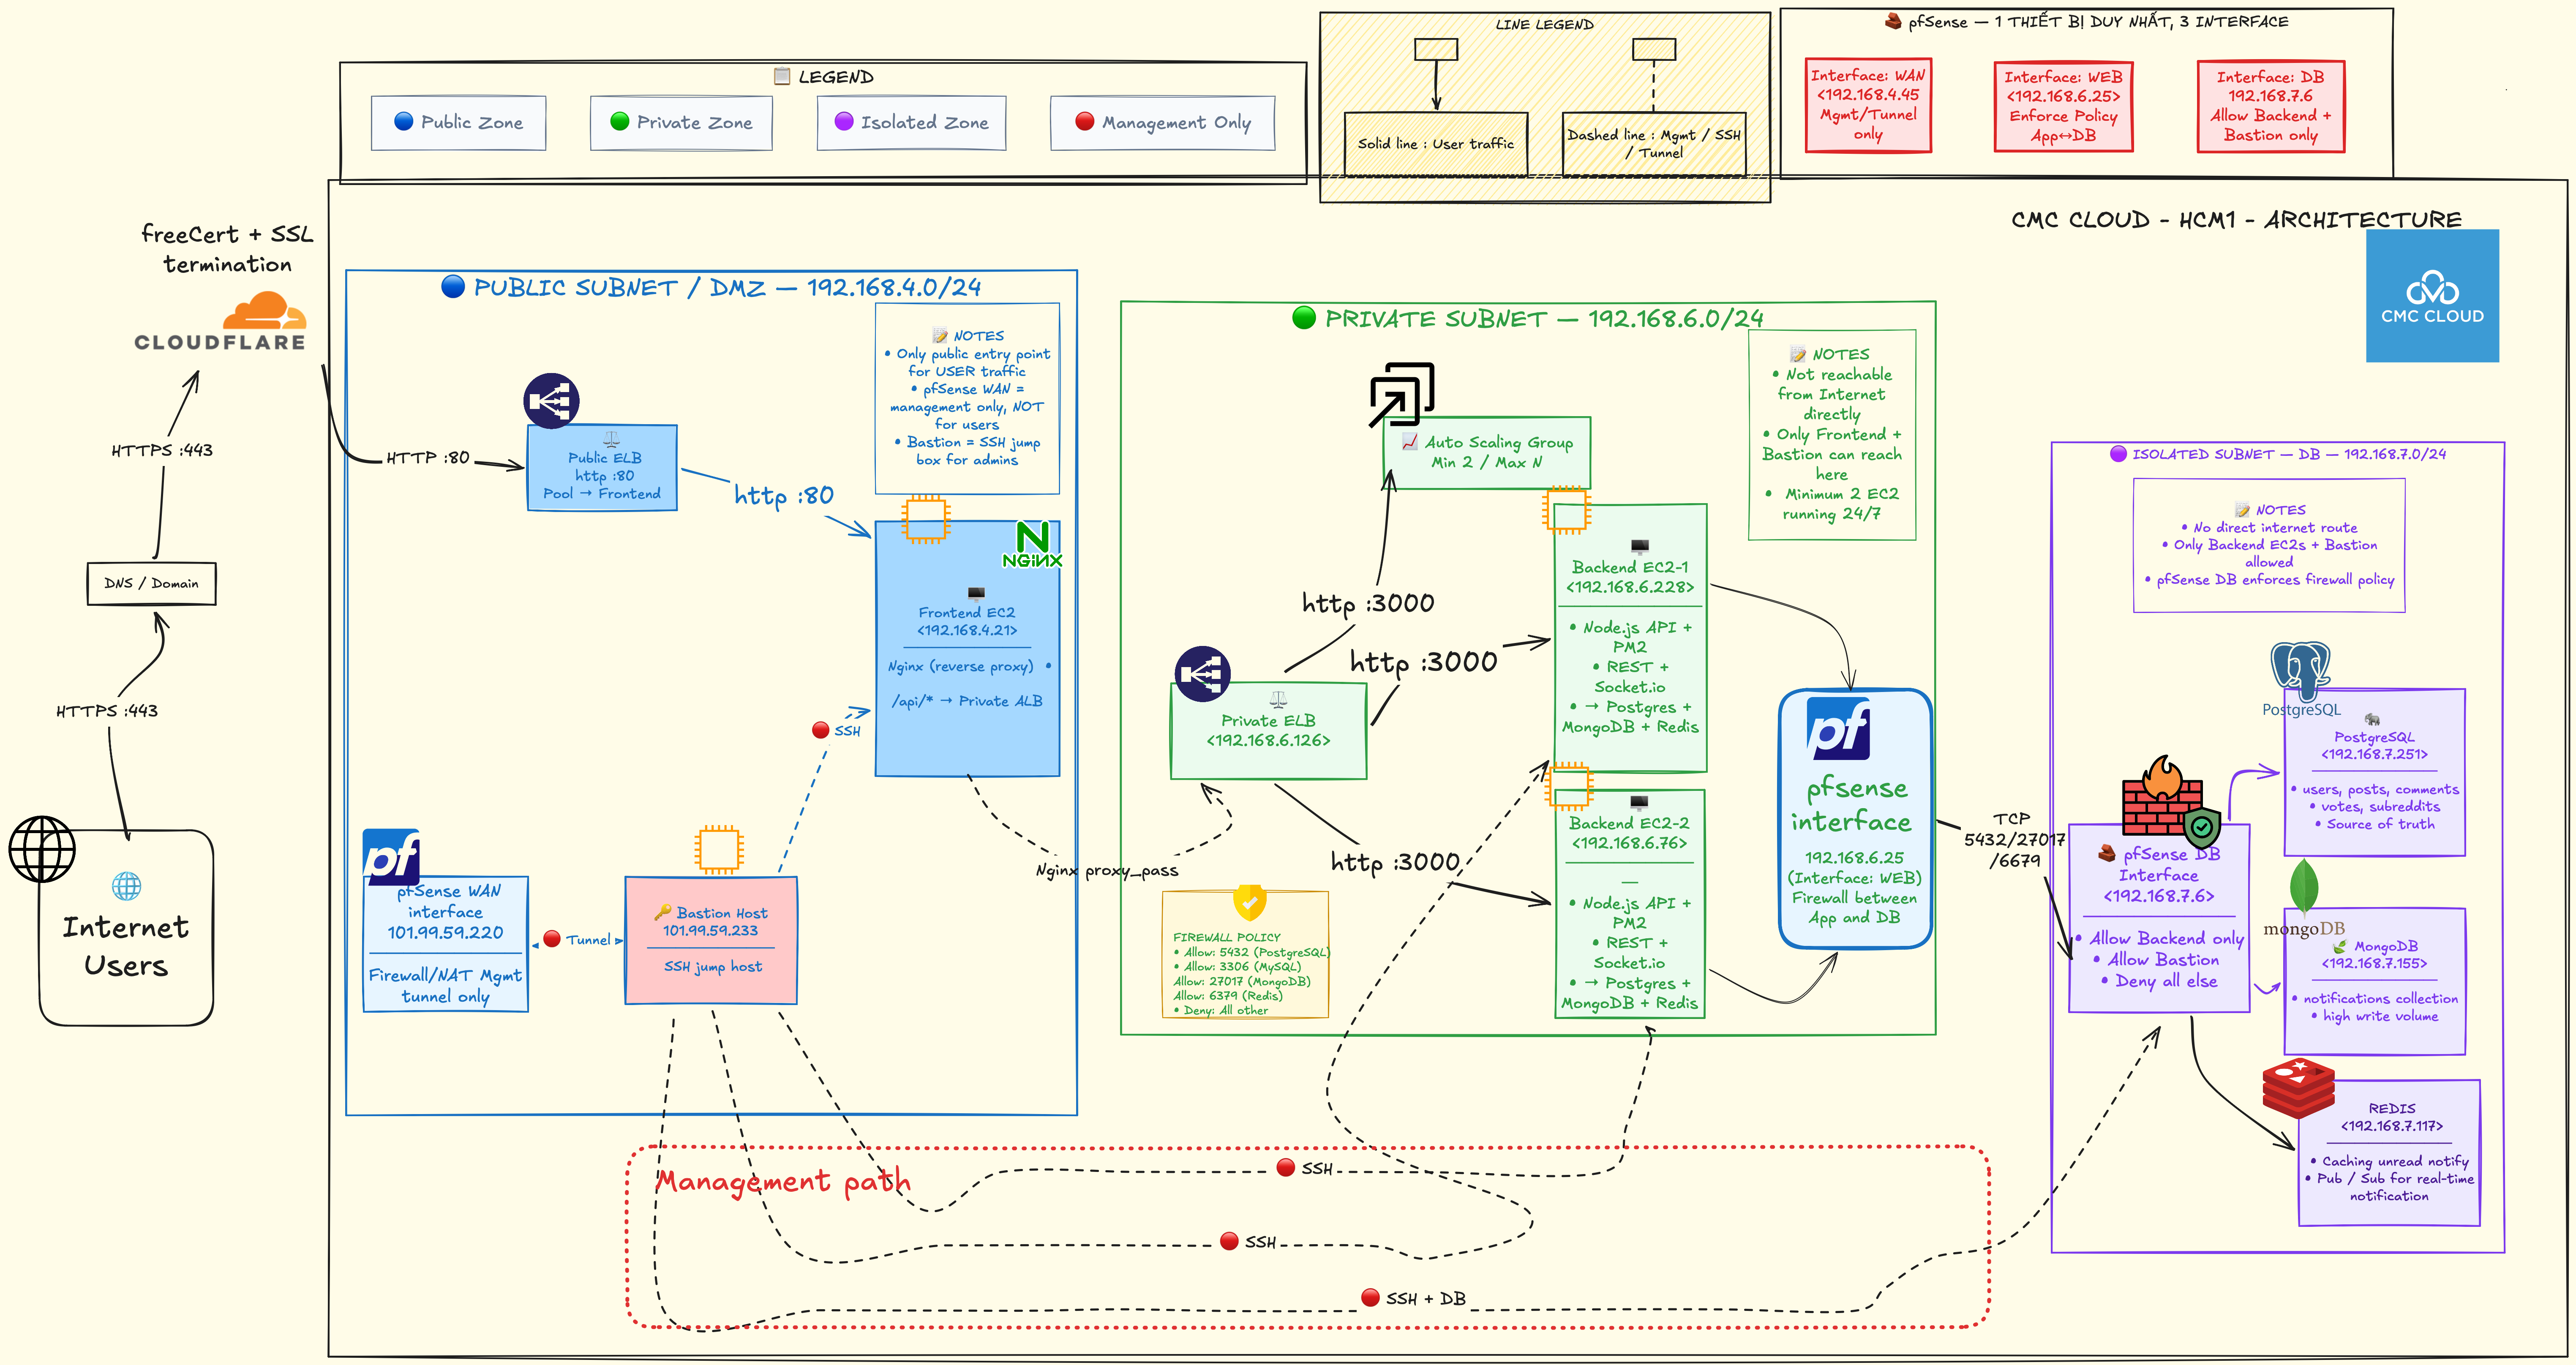
\includegraphics[width=0.9\textwidth]{architecture_guide/cmc-cloud-architecture.png}
  \caption{Sơ đồ kiến trúc hạ tầng và phân tầng cơ sở dữ liệu Clouddit trên CMC Cloud}
  \label{fig:hcm1_architecture}
\end{figure}

\begin{figure}[h!]
  \centering
  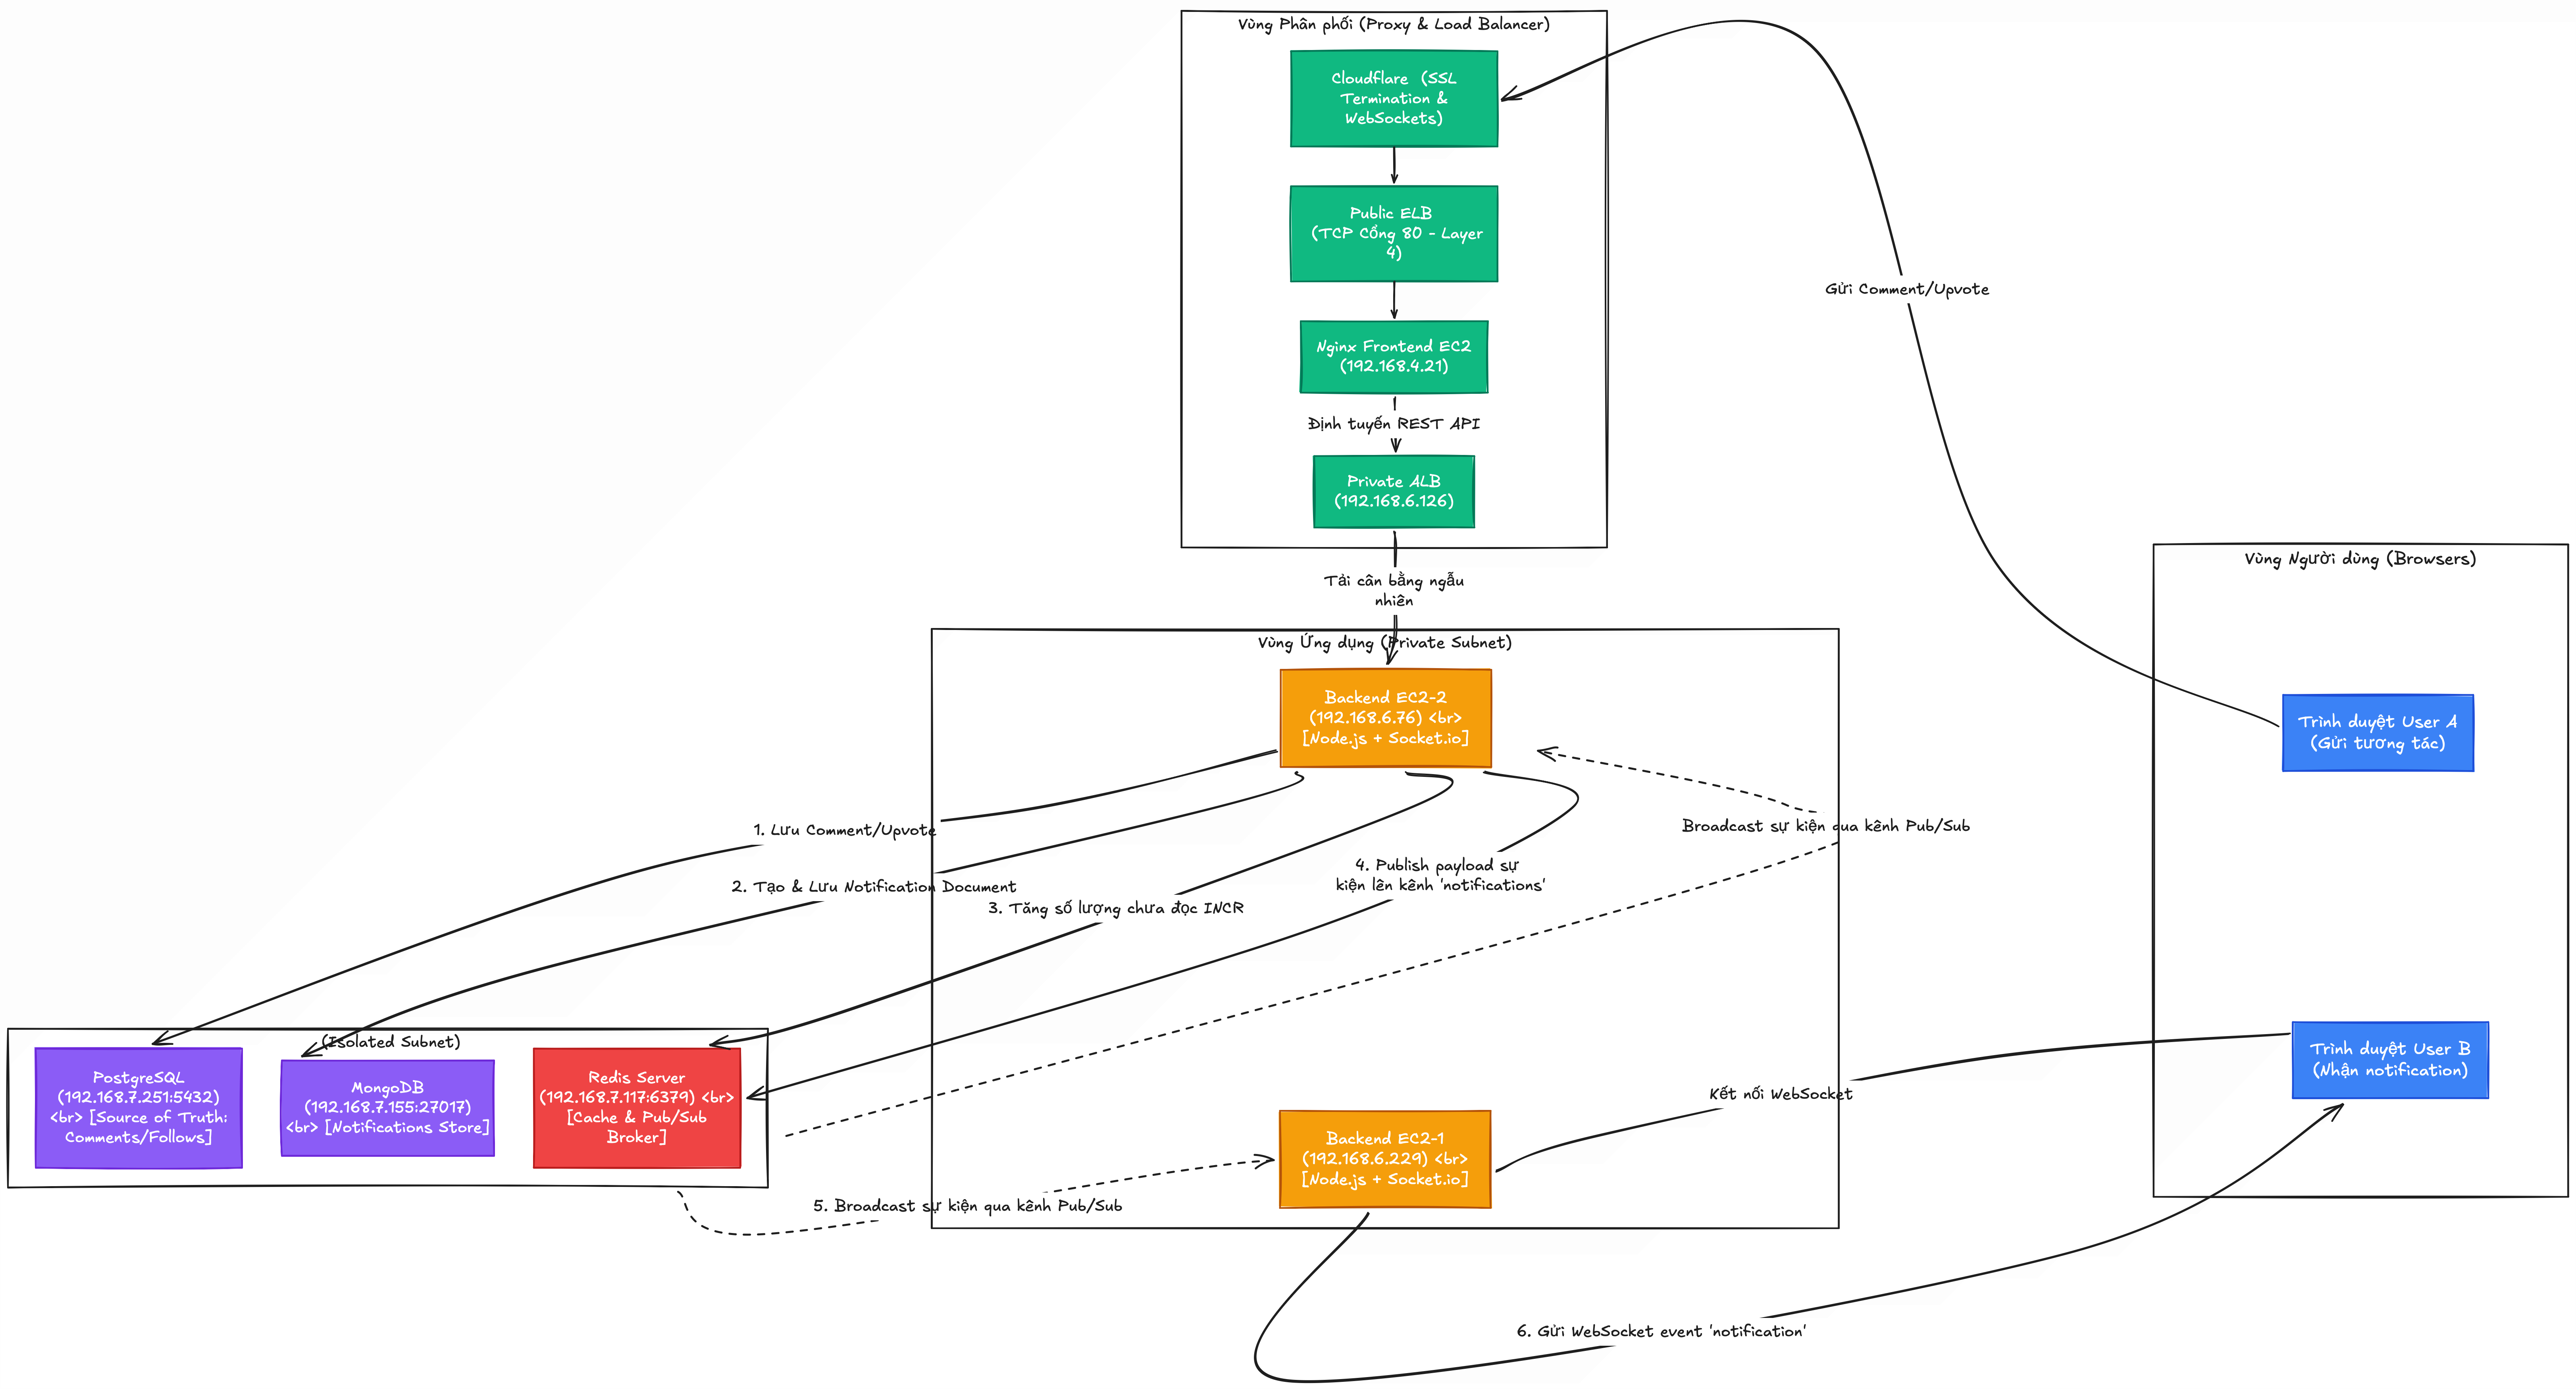
\includegraphics[width=0.9\textwidth]{architecture_guide/redis-pub-sub-work.png}
  \caption{Mô hình định tuyến và đồng bộ hóa WebSocket qua Redis Pub/Sub}
  \label{fig:redis_pubsub}
\end{figure}

\newpage
\section{Kết quả / Những gì đã học được}

\begin{itemize}
  \item Nắm vững quy trình thiết kế và cấu hình mạng VPC thực tế, phân chia subnet hợp lý để bảo vệ cơ sở dữ liệu.
  \item Làm chủ mô hình lưu trữ đa cơ sở dữ liệu (Polyglot Persistence): Sử dụng PostgreSQL cho tính nhất quán ACID, MongoDB cho log linh hoạt tốc độ ghi cao, và Redis cho đệm tốc độ truy vấn phản hồi nhanh (<1ms).
  \item Giải quyết triệt để bài toán đồng bộ hóa thời gian thực (Real-time Sync) trên cụm server co giãn thông qua cơ chế Redis Pub/Sub.
  \item Thực hành thành thạo các tính năng bảo mật nâng cao của Cloudflare (Proxy, WAF, SSL Full Mode) và cấu hình SSL Let's Encrypt trên Nginx.
  \item Có kỹ năng thực tiễn sử dụng k6 để thực hiện stress test các API có tải cao.
\end{itemize}

\section{Khó khăn / Vướng mắc}

\begin{itemize}
  \item Kết nối WebSocket bị đứt hoặc lỗi HTTP 400 Bad Request khi đi qua Load Balancer Layer 7 do ALB không tự nâng cấp giao thức nếu không cấu hình Session Sticky. Khắc phục bằng cách chuyển ELB sang Layer 4.
  \item MongoDB mặc định tiêu tốn nhiều dung lượng RAM khi lưu trữ log dài ngày, cần thiết lập Compound Index và TTL Index hợp lý để tự động dọn dẹp các bản ghi cũ.
  \item Sự cố crash của PM2 do thiếu biến môi trường trong tệp cấu hình khi deploy tự động, cần bổ sung reconnect loop để bảo vệ tiến trình.
\end{itemize}

\section{Kế hoạch tuần tới}

\begin{itemize}
  \item Thiết lập hệ thống CI/CD tự động hóa build và deploy ứng dụng Clouddit lên CMC Cloud sử dụng GitLab CI/CD.
  \item Cấu hình tính năng nhân bản cơ sở dữ liệu PostgreSQL (Read Replica) và cụm Redis Cluster để nâng cao tính sẵn sàng cao (High Availability).
  \item Triển khai hệ thống giám sát tập trung Prometheus và Grafana để theo dõi hiệu năng tài nguyên hệ thống (CPU, RAM, Disk I/O, Network traffic).
\end{itemize}

\end{document}